\documentclass[]{article}
\usepackage{lmodern}
\usepackage{amssymb,amsmath}
\usepackage{ifxetex,ifluatex}
\usepackage{fixltx2e} % provides \textsubscript
\ifnum 0\ifxetex 1\fi\ifluatex 1\fi=0 % if pdftex
  \usepackage[T1]{fontenc}
  \usepackage[utf8]{inputenc}
\else % if luatex or xelatex
  \ifxetex
    \usepackage{mathspec}
  \else
    \usepackage{fontspec}
  \fi
  \defaultfontfeatures{Ligatures=TeX,Scale=MatchLowercase}
\fi
% use upquote if available, for straight quotes in verbatim environments
\IfFileExists{upquote.sty}{\usepackage{upquote}}{}
% use microtype if available
\IfFileExists{microtype.sty}{%
\usepackage{microtype}
\UseMicrotypeSet[protrusion]{basicmath} % disable protrusion for tt fonts
}{}
\usepackage[margin=1in]{geometry}
\usepackage{hyperref}
\hypersetup{unicode=true,
            pdftitle={Estimating permutation p-values using MatrixEQTL},
            pdfborder={0 0 0},
            breaklinks=true}
\urlstyle{same}  % don't use monospace font for urls
\usepackage{color}
\usepackage{fancyvrb}
\newcommand{\VerbBar}{|}
\newcommand{\VERB}{\Verb[commandchars=\\\{\}]}
\DefineVerbatimEnvironment{Highlighting}{Verbatim}{commandchars=\\\{\}}
% Add ',fontsize=\small' for more characters per line
\usepackage{framed}
\definecolor{shadecolor}{RGB}{248,248,248}
\newenvironment{Shaded}{\begin{snugshade}}{\end{snugshade}}
\newcommand{\KeywordTok}[1]{\textcolor[rgb]{0.13,0.29,0.53}{\textbf{#1}}}
\newcommand{\DataTypeTok}[1]{\textcolor[rgb]{0.13,0.29,0.53}{#1}}
\newcommand{\DecValTok}[1]{\textcolor[rgb]{0.00,0.00,0.81}{#1}}
\newcommand{\BaseNTok}[1]{\textcolor[rgb]{0.00,0.00,0.81}{#1}}
\newcommand{\FloatTok}[1]{\textcolor[rgb]{0.00,0.00,0.81}{#1}}
\newcommand{\ConstantTok}[1]{\textcolor[rgb]{0.00,0.00,0.00}{#1}}
\newcommand{\CharTok}[1]{\textcolor[rgb]{0.31,0.60,0.02}{#1}}
\newcommand{\SpecialCharTok}[1]{\textcolor[rgb]{0.00,0.00,0.00}{#1}}
\newcommand{\StringTok}[1]{\textcolor[rgb]{0.31,0.60,0.02}{#1}}
\newcommand{\VerbatimStringTok}[1]{\textcolor[rgb]{0.31,0.60,0.02}{#1}}
\newcommand{\SpecialStringTok}[1]{\textcolor[rgb]{0.31,0.60,0.02}{#1}}
\newcommand{\ImportTok}[1]{#1}
\newcommand{\CommentTok}[1]{\textcolor[rgb]{0.56,0.35,0.01}{\textit{#1}}}
\newcommand{\DocumentationTok}[1]{\textcolor[rgb]{0.56,0.35,0.01}{\textbf{\textit{#1}}}}
\newcommand{\AnnotationTok}[1]{\textcolor[rgb]{0.56,0.35,0.01}{\textbf{\textit{#1}}}}
\newcommand{\CommentVarTok}[1]{\textcolor[rgb]{0.56,0.35,0.01}{\textbf{\textit{#1}}}}
\newcommand{\OtherTok}[1]{\textcolor[rgb]{0.56,0.35,0.01}{#1}}
\newcommand{\FunctionTok}[1]{\textcolor[rgb]{0.00,0.00,0.00}{#1}}
\newcommand{\VariableTok}[1]{\textcolor[rgb]{0.00,0.00,0.00}{#1}}
\newcommand{\ControlFlowTok}[1]{\textcolor[rgb]{0.13,0.29,0.53}{\textbf{#1}}}
\newcommand{\OperatorTok}[1]{\textcolor[rgb]{0.81,0.36,0.00}{\textbf{#1}}}
\newcommand{\BuiltInTok}[1]{#1}
\newcommand{\ExtensionTok}[1]{#1}
\newcommand{\PreprocessorTok}[1]{\textcolor[rgb]{0.56,0.35,0.01}{\textit{#1}}}
\newcommand{\AttributeTok}[1]{\textcolor[rgb]{0.77,0.63,0.00}{#1}}
\newcommand{\RegionMarkerTok}[1]{#1}
\newcommand{\InformationTok}[1]{\textcolor[rgb]{0.56,0.35,0.01}{\textbf{\textit{#1}}}}
\newcommand{\WarningTok}[1]{\textcolor[rgb]{0.56,0.35,0.01}{\textbf{\textit{#1}}}}
\newcommand{\AlertTok}[1]{\textcolor[rgb]{0.94,0.16,0.16}{#1}}
\newcommand{\ErrorTok}[1]{\textcolor[rgb]{0.64,0.00,0.00}{\textbf{#1}}}
\newcommand{\NormalTok}[1]{#1}
\usepackage{graphicx,grffile}
\makeatletter
\def\maxwidth{\ifdim\Gin@nat@width>\linewidth\linewidth\else\Gin@nat@width\fi}
\def\maxheight{\ifdim\Gin@nat@height>\textheight\textheight\else\Gin@nat@height\fi}
\makeatother
% Scale images if necessary, so that they will not overflow the page
% margins by default, and it is still possible to overwrite the defaults
% using explicit options in \includegraphics[width, height, ...]{}
\setkeys{Gin}{width=\maxwidth,height=\maxheight,keepaspectratio}
\IfFileExists{parskip.sty}{%
\usepackage{parskip}
}{% else
\setlength{\parindent}{0pt}
\setlength{\parskip}{6pt plus 2pt minus 1pt}
}
\setlength{\emergencystretch}{3em}  % prevent overfull lines
\providecommand{\tightlist}{%
  \setlength{\itemsep}{0pt}\setlength{\parskip}{0pt}}
\setcounter{secnumdepth}{0}
% Redefines (sub)paragraphs to behave more like sections
\ifx\paragraph\undefined\else
\let\oldparagraph\paragraph
\renewcommand{\paragraph}[1]{\oldparagraph{#1}\mbox{}}
\fi
\ifx\subparagraph\undefined\else
\let\oldsubparagraph\subparagraph
\renewcommand{\subparagraph}[1]{\oldsubparagraph{#1}\mbox{}}
\fi

%%% Use protect on footnotes to avoid problems with footnotes in titles
\let\rmarkdownfootnote\footnote%
\def\footnote{\protect\rmarkdownfootnote}

%%% Change title format to be more compact
\usepackage{titling}

% Create subtitle command for use in maketitle
\providecommand{\subtitle}[1]{
  \posttitle{
    \begin{center}\large#1\end{center}
    }
}

\setlength{\droptitle}{-2em}

  \title{Estimating permutation p-values using MatrixEQTL}
    \pretitle{\vspace{\droptitle}\centering\huge}
  \posttitle{\par}
    \author{}
    \preauthor{}\postauthor{}
    \date{}
    \predate{}\postdate{}
  

\begin{document}
\maketitle

The basic pipeline includes data preparation steps:

1 step0\_submit\_trim.R - trimming suspicious allele-specific counts and
total counts 2 step1\_submit\_preprocSNP.R - creating separate files for
each gene

main eQTL analysis and p-value estimate:

3 step2\_submit\_trecaseA.R 4 step4\_submit\_MatrixEQTL.R

and further analysis steps including principal component analysis and
dynamic eqtl findigs.

Once the specification file is set up, each script should be able to be
run authomatically (with corresponding note given to the script to
distinguish between long and short model, etc)

1 Exact code to be run: R CMD BATCH `--args
specifications\_Muscle\_Skeletal.txt long' step0\_submit\_trim.R
MS\_step0\_submit\_trim\_long.Rout

1.a To save time short model fit relies on long model being run first,
so this step should be done after the previous is completed. R CMD BATCH
`--args specifications\_Muscle\_Skeletal.txt short'
step0\_submit\_trim.R MS\_step0\_submit\_trim\_short.Rout 2 wait until
the previous step completes R CMD BATCH `--args
specifications\_Muscle\_Skeletal.txt' step1\_submit\_preprocSNP.R
MS\_step1\_submit\_preprocSNP.Rout 3 wait until the previous step
completes fitting steps can be run at once, if you have generous enough
scheduler (often schedulers have limit on the number of maximum number
of jobs that can be submitted) fitting TReCASE model for each gene, long
model: R CMD BATCH `--args specifications\_Muscle\_Skeletal.txt long
5e5' step2\_submit\_trecaseA.R MS\_step2\_submit\_trecaseA\_long.Rout R
CMD BATCH `--args specifications\_Muscle\_Skeletal.txt short 5e5'
step2\_submit\_trecaseA.R MS\_step2\_submit\_trecaseA\_short.Rout 4
estimating permuted p-values R CMD BATCH `--args
specifications\_Muscle\_Skeletal.txt long 5e5'
step4\_submit\_MatrixEQTL.R MS\_step4\_submit\_MatrixEQTL\_long.Rout R
CMD BATCH `--args specifications\_Muscle\_Skeletal.txt short 5e5'
step4\_submit\_MatrixEQTL.R MS\_step4\_submit\_MatrixEQTL\_short.Rout

Assuming, that previous step reformatting the data is finished,
step4\_MatrixEQTL script will submit each gene to produce runs multiple
bootstraps to estimate permutation p-value.

step4\_submitMatrixEQTL.R will call step4\_MatrixEQTL.R with several
options: chromosome (in this example 9), number of samples inthe dataset
(this can be taken from specification file) random seed 1565691 window -
5e+05 is used in this example and which model is used - shorter model
for this example and optional parameter - how much paralellization you
want to introduce (if your cluster supports submitting multiple jobs,
for this example set to 1 meaning that every job will be run
sequentially)

\begin{Shaded}
\begin{Highlighting}[]
\NormalTok{com =}\StringTok{ }\KeywordTok{sprintf}\NormalTok{(}\StringTok{"R CMD BATCH  }\CharTok{\textbackslash{}"}\StringTok{--args specifications_Muscle_Skeletal.txt short 5e5}\CharTok{\textbackslash{}"}\StringTok{ step4_submit_MatrixEQTL.R MS_step4_submit_MatrixEQTL_short.Rout"}\NormalTok{)}
\KeywordTok{message}\NormalTok{(com)}
\end{Highlighting}
\end{Shaded}

\begin{verbatim}
## R CMD BATCH  "--args specifications_Muscle_Skeletal.txt short 5e5" step4_submit_MatrixEQTL.R MS_step4_submit_MatrixEQTL_short.Rout
\end{verbatim}

\begin{Shaded}
\begin{Highlighting}[]
\KeywordTok{system}\NormalTok{(com)}
\end{Highlighting}
\end{Shaded}

Lets illustrate calculation of permutation p-value estimate. We take the
values generated in step4\_runboot.R and fit glm predicting probability
of observing more extreme result (then observed in bootstrap) by
log10(minimum p-value). After fitting glm, predict permutation p-value
based on log10(minimum p-value) Effective number of tests will be ratio
of predicted permutation p-value and minimum p-value (trimmed between 1
and number of SNPs)

\begin{Shaded}
\begin{Highlighting}[]
\KeywordTok{setwd}\NormalTok{(}\StringTok{"C:/Users/Vasyl/Documents/GitHub/asSeq/pipeline_GTEx/v8/example/Muscle_Skeletal"}\NormalTok{)}
\NormalTok{perm.dir =}\StringTok{ "boot_Muscle_Skeletal_704_5e+05_short_100"}
\NormalTok{out.dir =}\StringTok{ }\KeywordTok{sprintf}\NormalTok{(}\StringTok{"oneperm_Muscle_Skeletal_704_5e+05_short"}\NormalTok{)}
\NormalTok{logiti =}\StringTok{ }\ControlFlowTok{function}\NormalTok{(x)}\DecValTok{1}\OperatorTok{/}\NormalTok{(}\DecValTok{1}\OperatorTok{+}\KeywordTok{exp}\NormalTok{(}\OperatorTok{-}\NormalTok{x))}


\NormalTok{boots =}\StringTok{ }\KeywordTok{read.csv}\NormalTok{(}\KeywordTok{sprintf}\NormalTok{(}\StringTok{"%s/short_boot_pval_9_1.csv"}\NormalTok{, perm.dir), }\DataTypeTok{as.is=}\NormalTok{T)}
\NormalTok{eigenMT =}\StringTok{ }\KeywordTok{read.csv}\NormalTok{(}\KeywordTok{sprintf}\NormalTok{(}\StringTok{"%s/upd_eigenMT_9_1.csv"}\NormalTok{, out.dir), }\DataTypeTok{as.is=}\NormalTok{T)}
\NormalTok{nperm =}\StringTok{ }\DecValTok{1000}
\NormalTok{y =}\StringTok{ }\NormalTok{boots}\OperatorTok{$}\NormalTok{permp}\OperatorTok{*}\NormalTok{nperm}
\NormalTok{pvalb =}\StringTok{ }\NormalTok{boots}\OperatorTok{$}\NormalTok{pvalb}
\NormalTok{kp3 =}\StringTok{ }\NormalTok{(y}\OperatorTok{/}\NormalTok{nperm)}\OperatorTok{>=}\DecValTok{0}     \OperatorTok{&}\StringTok{ }\NormalTok{(y}\OperatorTok{/}\NormalTok{nperm)}\OperatorTok{<=}\FloatTok{0.3}
\NormalTok{kp3a =}\StringTok{ }\NormalTok{(y}\OperatorTok{/}\NormalTok{nperm)}\OperatorTok{>}\DecValTok{0}     \OperatorTok{&}\StringTok{ }\NormalTok{(y}\OperatorTok{/}\NormalTok{nperm)}\OperatorTok{<=}\FloatTok{0.3}
    
\NormalTok{y1 =}\StringTok{ }\KeywordTok{log10}\NormalTok{(y}\OperatorTok{/}\NormalTok{nperm)}
\NormalTok{x1 =}\StringTok{ }\KeywordTok{log10}\NormalTok{(pvalb)}
\NormalTok{glmi3 =}\StringTok{ }\KeywordTok{glm}\NormalTok{(}\KeywordTok{cbind}\NormalTok{(y[kp3],nperm}\OperatorTok{-}\NormalTok{y[kp3])}\OperatorTok{~}\NormalTok{x1[kp3], }\DataTypeTok{family=}\StringTok{"binomial"}\NormalTok{)}
\KeywordTok{summary}\NormalTok{(glmi3)}
\end{Highlighting}
\end{Shaded}

\begin{verbatim}
## 
## Call:
## glm(formula = cbind(y[kp3], nperm - y[kp3]) ~ x1[kp3], family = "binomial")
## 
## Deviance Residuals: 
##     Min       1Q   Median       3Q      Max  
## -3.2386  -0.7024  -0.0964   0.6726   2.3370  
## 
## Coefficients:
##             Estimate Std. Error z value Pr(>|z|)    
## (Intercept)  5.32658    0.12261   43.45   <2e-16 ***
## x1[kp3]      2.07455    0.03285   63.16   <2e-16 ***
## ---
## Signif. codes:  0 '***' 0.001 '**' 0.01 '*' 0.05 '.' 0.1 ' ' 1
## 
## (Dispersion parameter for binomial family taken to be 1)
## 
##     Null deviance: 6555.17  on 98  degrees of freedom
## Residual deviance:  102.31  on 97  degrees of freedom
## AIC: 559.99
## 
## Number of Fisher Scoring iterations: 4
\end{verbatim}

\begin{Shaded}
\begin{Highlighting}[]
\NormalTok{xval =}\StringTok{ }\KeywordTok{log10}\NormalTok{(eigenMT}\OperatorTok{$}\NormalTok{p.value)}
\NormalTok{pred.perm =}\StringTok{ }\KeywordTok{logiti}\NormalTok{(glmi3}\OperatorTok{$}\NormalTok{coef[}\DecValTok{1}\NormalTok{]}\OperatorTok{+}\NormalTok{glmi3}\OperatorTok{$}\NormalTok{coef[}\DecValTok{2}\NormalTok{]}\OperatorTok{*}\NormalTok{xval)}
\KeywordTok{c}\NormalTok{(xval, pred.perm)}
\end{Highlighting}
\end{Shaded}

\begin{verbatim}
##                 (Intercept) 
## -3.906636e+01  1.305708e-33
\end{verbatim}

\begin{Shaded}
\begin{Highlighting}[]
\NormalTok{xlim =}\StringTok{ }\KeywordTok{range}\NormalTok{(}\OperatorTok{-}\KeywordTok{c}\NormalTok{(x1, xval))}
\NormalTok{ylim =}\StringTok{ }\KeywordTok{range}\NormalTok{(}\OperatorTok{-}\KeywordTok{log10}\NormalTok{(y}\OperatorTok{/}\NormalTok{nperm))}
\NormalTok{ylim[}\DecValTok{2}\NormalTok{] =}\StringTok{ }\OperatorTok{-}\KeywordTok{log10}\NormalTok{(pred.perm)}

\KeywordTok{plot}\NormalTok{(}\OperatorTok{-}\NormalTok{x1, }\OperatorTok{-}\KeywordTok{log10}\NormalTok{(y}\OperatorTok{/}\NormalTok{nperm), }\DataTypeTok{xlab=}\StringTok{"-log10(boot p-val)"}\NormalTok{, }\DataTypeTok{ylab=}\StringTok{"permutation p-val"}\NormalTok{, }\DataTypeTok{bty=}\StringTok{"n"}\NormalTok{, }\DataTypeTok{main=}\StringTok{"perm.p vs min.p"}\NormalTok{)}
\NormalTok{o =}\StringTok{ }\KeywordTok{order}\NormalTok{(x1[kp3])}
\NormalTok{xf =}\StringTok{ }\NormalTok{x1[kp3][o]}
\NormalTok{yf =}\StringTok{ }\NormalTok{glmi3}\OperatorTok{$}\NormalTok{fitted.values[o]}
\KeywordTok{lines}\NormalTok{(}\OperatorTok{-}\NormalTok{xf, }\OperatorTok{-}\KeywordTok{log10}\NormalTok{(yf), }\DataTypeTok{col=}\StringTok{"red"}\NormalTok{)}
\end{Highlighting}
\end{Shaded}

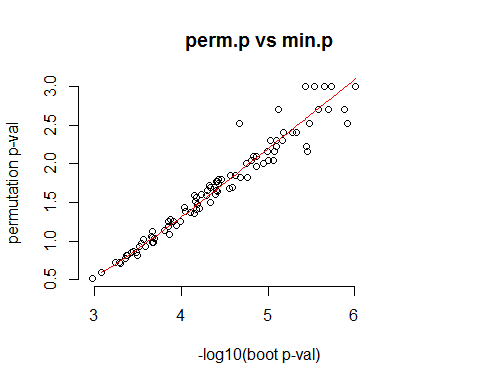
\includegraphics{estimating_permPshort_files/figure-latex/illustrate estimate-1.pdf}

\begin{Shaded}
\begin{Highlighting}[]
\NormalTok{fit =}\StringTok{ }\KeywordTok{seq}\NormalTok{(}\DecValTok{0}\NormalTok{, xval, }\DataTypeTok{length.out=}\DecValTok{50}\NormalTok{)}
\NormalTok{pred.perm0 =}\StringTok{ }\KeywordTok{logiti}\NormalTok{(glmi3}\OperatorTok{$}\NormalTok{coef[}\DecValTok{1}\NormalTok{]}\OperatorTok{+}\NormalTok{glmi3}\OperatorTok{$}\NormalTok{coef[}\DecValTok{2}\NormalTok{]}\OperatorTok{*}\NormalTok{fit)}
\KeywordTok{plot}\NormalTok{(}\OperatorTok{-}\NormalTok{x1, }\OperatorTok{-}\KeywordTok{log10}\NormalTok{(y}\OperatorTok{/}\NormalTok{nperm), }\DataTypeTok{xlab=}\StringTok{"-log10(boot p-val)"}\NormalTok{, }\DataTypeTok{ylab=}\StringTok{"permutation p-val"}\NormalTok{, }\DataTypeTok{bty=}\StringTok{"n"}\NormalTok{, }\DataTypeTok{main=}\StringTok{"perm.p vs min.p"}\NormalTok{, }\DataTypeTok{xlim=}\NormalTok{xlim,}\DataTypeTok{ylim=}\NormalTok{ylim)}
\KeywordTok{lines}\NormalTok{(}\OperatorTok{-}\NormalTok{fit, }\OperatorTok{-}\KeywordTok{log10}\NormalTok{(pred.perm0), }\DataTypeTok{col=}\StringTok{"red"}\NormalTok{)}
\KeywordTok{points}\NormalTok{(}\OperatorTok{-}\NormalTok{xval, }\OperatorTok{-}\KeywordTok{log10}\NormalTok{(pred.perm), }\DataTypeTok{col=}\StringTok{"blue"}\NormalTok{, }\DataTypeTok{cex=}\DecValTok{1}\NormalTok{, }\DataTypeTok{pch=}\DecValTok{19}\NormalTok{)}
\KeywordTok{legend}\NormalTok{(}\StringTok{"topleft"}\NormalTok{, }\StringTok{"estimated permu.p"}\NormalTok{, }\DataTypeTok{text.col=}\StringTok{"blue"}\NormalTok{, }\DataTypeTok{pch=}\DecValTok{19}\NormalTok{, }\DataTypeTok{col=}\StringTok{"blue"}\NormalTok{, }\DataTypeTok{bty=}\StringTok{"n"}\NormalTok{)                 }
\end{Highlighting}
\end{Shaded}

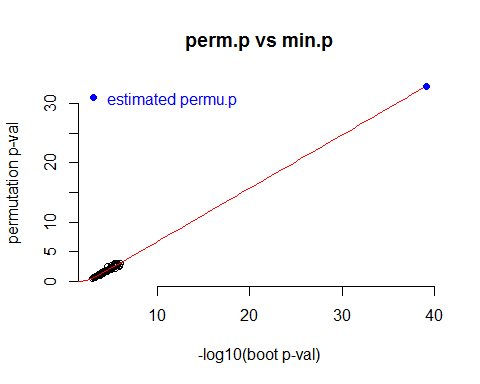
\includegraphics{estimating_permPshort_files/figure-latex/illustrate estimate-2.pdf}


\end{document}
